\documentclass{beamer}
\usepackage[utf8]{inputenc}
\usepackage{multirow}
\usepackage{colortbl}
\usepackage{tikz}
\usepackage{amsmath}
% \usepackage{anyfontsize}
% \usepackage{lmodern}
%\usepackage{svg}

\usetheme[
titlepagelogo=img/logo_unimib.pdf,
color=red,
language=italian,
bullet=triangle,
coding=utf8,
pageofpages=di,
assistantsupervisor=true
]{TorinoTh}
\author{Giacomini Stefano}
\rel{Prof. Gianluca Della Vedova}
\title{Simulated Annealing per l'inferenza di mutazioni\\ ricorrenti in alberi tumorali}
\ateneo{Università degli Studi di Milano-Bicocca}
\date{21 Marzo 2022}
\assistantsupervisor{Dott. Simone Ciccolella}

% \usepackage[dvipsnames]{xcolor}

% \definecolor{darkgreen}{RGB}{20, 155, 82}
% \definecolor{moredarkgreen}{RGB}{14, 84, 46}
\usepackage[beamer,customcolors]{hf-tikz}
\hfsetfillcolor{alerted text.fg!10}
\hfsetbordercolor{alerted text.fg}
\begin{document}
\titlepageframe

\begin{tframe}{Introduzione e scaletta}
  \begin{block}<1->{Introduzione e motivazioni:}
    \begin{itemize}
      \item terapia mirata per la cura di tumori
      \item importanza dell'omoplasia nei dati virali
    \end{itemize}
  \end{block}
  \begin{block}<2->{{Definizioni e aggiunte:}}
    \begin{itemize}
      \item Problemi di riscostruzione di alberi filogenetici
      \item Dollo-k e Camin-Sokal-k
      \item Simulated Annealing
      \item Aggiunte del codice
      \item Analisi dei tempi
    \end{itemize}
  \end{block}
\end{tframe}

\begin{tframe}{Definizioni: Problema di riscostruzione di alberi filogenetici}
    \vspace{5mm}
    \begin{itemize}
      \item \textit{matrice di input}
      \item \textit{nuovi nodi e regole}
      \item \textit{profilo del genotipo}
    \end{itemize}

    \vspace{10mm}
    \tiny
    \begin{equation*}
      \tikzmarkin<1->{a}(0.2,-0.4)(-0.2,0.45)
        \max{\sum_{j}^{m}[-c_{j}\log(1-P(L(j)))-f_{j}\log(1-P(D(j)))+\sum_{i}^{n}\log(P(I_{ij}|D(T, \sigma_{i})_{j}))]}
      \tikzmarkend{a}
    \end{equation*}
\end{tframe}

\begin{tframe}{Definizioni: Dollo-k e Camin-Sokal-k}
  \begin{columns}
  \column{0.35\textwidth}
  \begin{itemize}
    \item \textit{Dollo}
    \item \textit{Camin-Sokal}
    \item \textit{modello utilizzato}
  \end{itemize}


  \column{0.55\textwidth}
  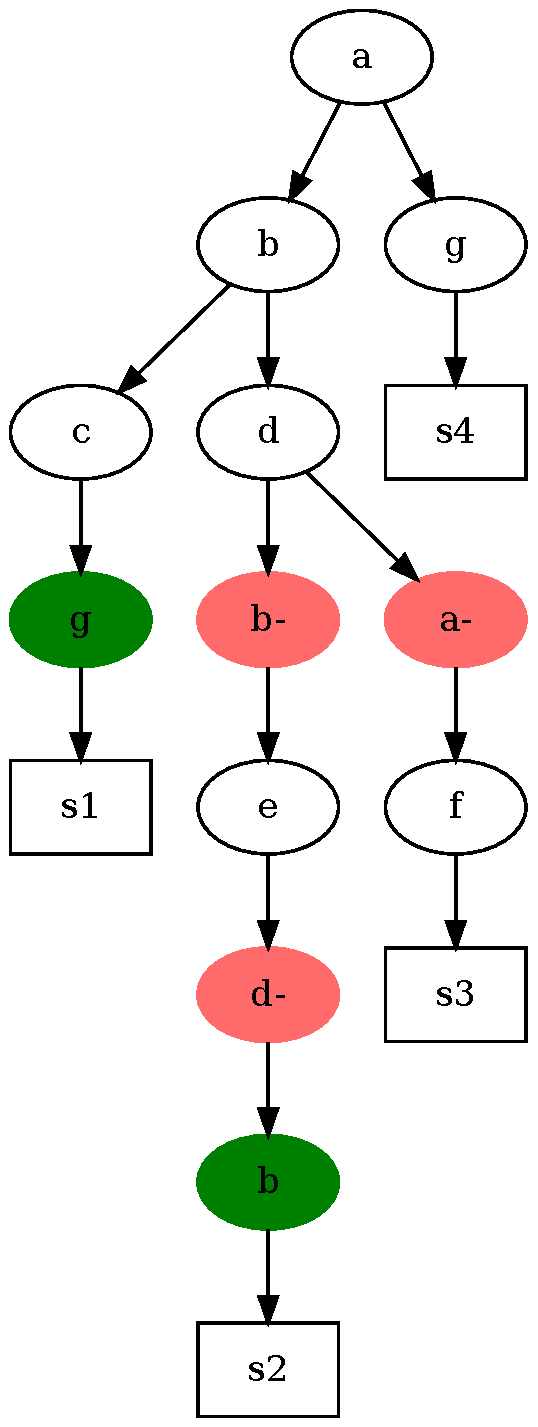
\includegraphics[scale = 0.23]{img/tree.pdf}
\end{columns}
\end{tframe}

\begin{tframe}{Definizioni: Simulated Annealing}
  \begin{block}<1->{\ }
    \begin{itemize}
      \item funzionamento dell'algoritmo
      \item metodo di riduzione della temperatura
      \item mosse
    \end{itemize}
  \end{block}
\end{tframe}

\begin{tframe}{Aggiunte del codice}
  \begin{block}<1->{Aggiunte e modifiche fatte al codice}
    \begin{itemize}
      \item likelihood
      \item funzioni di creazione nodi speciali
      \item funzione di controllo
      \item test
    \end{itemize}
  \end{block}
\end{tframe}

\begin{tframe}{Analisi dei tempi e conclusioni}
  \begin{itemize}
    \item \textit{confronto media dei tempi con t-test}
    \item \textit{confronto dei tempi senza limiti al numero di nodi speciali}
  \end{itemize}

  \vspace{15mm}
  \centering
  \begin{columns}
    \column{0.2\textwidth}
    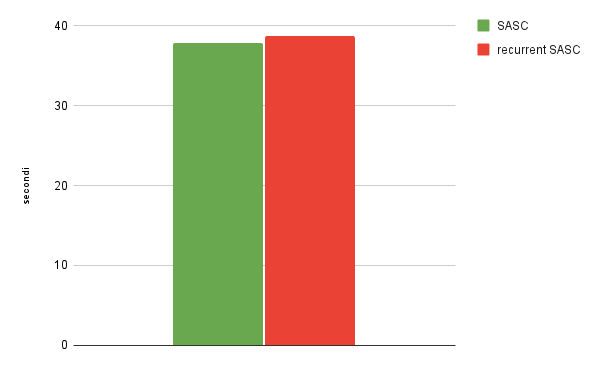
\includegraphics[scale = 0.2]{img/time1.png}

    \column{0.3\textwidth}
    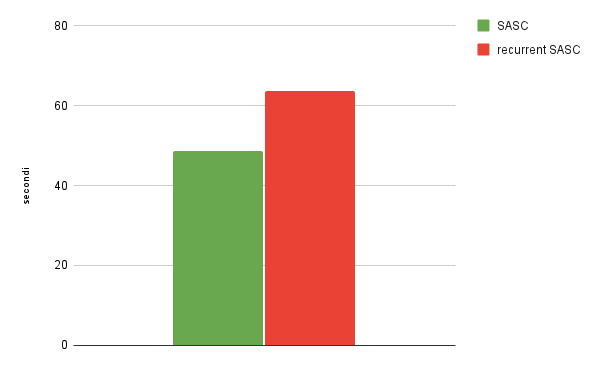
\includegraphics[scale = 0.2]{img/time2.png}
  \end{columns}
\end{tframe}

\title{Grazie per l'attenzione}
\ateneo{Ringraziamenti}
\titlepageframe

\end{document}
